% ============================================================================
% Section 5 — Experimental Results
% Paper review: Stealthy Computational Delay Attacks on Control Systems (ICCPS 2025)
% Compile:  pdflatex section5.tex   (run twice for the page numbers)
% Figures 2-4 and Table 1 in figs/ are from the paper, shown with citation.
% ============================================================================
\documentclass[aspectratio=169,10pt]{beamer}
\usetheme{default}
\usepackage[T1]{fontenc}
\usepackage[utf8]{inputenc}
\usepackage{graphicx}
\usepackage{xcolor}
\usepackage{amsmath}

% ---- colours (deck house style) ----
\definecolor{navy}{HTML}{15213B}
\definecolor{red}{HTML}{C0392B}
\definecolor{teal}{HTML}{2A7F7A}
\definecolor{gold}{HTML}{D9A441}
\definecolor{muted}{HTML}{4A5876}
\definecolor{light}{HTML}{F3F5F9}

\setbeamertemplate{navigation symbols}{}
\setbeamercolor{frametitle}{bg=navy,fg=white}
\setbeamerfont{frametitle}{series=\bfseries,size=\large}
\setbeamercolor{framesubtitle}{fg=red}
\setbeamerfont{framesubtitle}{shape=\itshape,size=\small}
\setbeamercolor{block title}{bg=navy,fg=white}
\setbeamercolor{block body}{bg=light,fg=black}
\setbeamercolor{itemize item}{fg=muted}
\setbeamercolor{itemize subitem}{fg=muted}
\setbeamercolor{normal text}{fg=black}
\setbeamerfont{block title}{size=\small,series=\bfseries}

% ---- footer: citation + frame number ----
\setbeamertemplate{footline}{%
  \hbox{\begin{beamercolorbox}[wd=\paperwidth,ht=2.2ex,dp=1ex,leftskip=.3cm,rightskip=.3cm]{}%
  {\color{muted}\tiny Source: Nauta, Sandberg \& Maggio, ``Stealthy Computational Delay Attacks on Control Systems,'' ICCPS 2025 $\cdot$ \S5 $\cdot$ DOI 10.1145/3716550.3722013}%
  \hfill{\color{muted}\tiny\insertframenumber}%
  \end{beamercolorbox}}}

\newcommand{\hook}[1]{\medskip{\footnotesize\textbf{\textcolor{gold}{$\rightarrow$ Extension hook:} }\textcolor{red}{\itshape #1}}}
\newcommand{\discuss}[1]{{\footnotesize\textbf{\textcolor{navy}{Discuss:} }\textcolor{muted}{#1}}}
\newcommand{\citefig}[1]{{\color{muted}\tiny Figure #1 $\cdot$ \copyright\ ACM --- Nauta, Sandberg \& Maggio, ICCPS 2025}}

\begin{document}

% ---------- 1. DIVIDER ----------
{\setbeamercolor{background canvas}{bg=navy}
\begin{frame}[plain]
  \vfill
  \centering
  {\color{gold}\large\textbf{SECTION 5}}\\[1.2em]
  {\color{white}\Huge\textbf{Experimental Results}}\\[1.0em]
  {\color{light}\large\itshape The paper's plots, discussed --- and where they open the door to our extension}\\[1.2em]
  {\color{muted}\normalsize Quadruple-tank (\S5.2) $\cdot$ Furuta pendulum (\S5.3) $\cdot$ Figures 2--4 $\cdot$ Table 1}
  \vfill
\end{frame}}

% ---------- 2. SETUP ----------
\begin{frame}{How the experiments are run}{\S5.1 \quad The MIQCP attacker on two benchmark plants}
  \begin{columns}[T]
    \begin{column}{0.56\textwidth}
      \begin{block}{Optimisation}
        A Mixed-Integer Quadratically-Constrained Program (MIQCP) in Gurobi (\texttt{gurobipy}), with indicator constraints for the hit/miss dynamics.
      \end{block}
      \begin{block}{What is measured}
        Per configuration: the optimal attack schedule, the optimal and nominal objectives, and effectiveness $\omega = J_{\text{attack}} - J_{\text{nominal}}$.
      \end{block}
    \end{column}
    \begin{column}{0.42\textwidth}
      \textbf{\textcolor{navy}{Swept parameters}}
      \begin{itemize}
        \item attack horizon $\ell \in \{1,\dots,25\}$
        \item watchdog threshold $\bar a \in \{1,\dots,5\}$
        \item detection window $n_w \in \{10,\dots,20\}$
        \item nominal miss prob.\ $\hat p_{\mathrm m} \in \{0.01,\dots,0.25\}$
        \item detector: binomial $\cdot$ $\chi^2$ $\cdot$ combined
      \end{itemize}
    \end{column}
  \end{columns}
  \medskip
  {\footnotesize\textcolor{red}{\textbf{Note:}} the full sweep is expensive (hours--days with a Gurobi licence).}
\end{frame}

% ---------- 3. QUAD TANK ----------
\begin{frame}{Quadruple-tank process}{\S5.2 \quad System A --- stable, non-minimum-phase, simulated (HOLD)}
  \begin{columns}[T]
    \begin{column}{0.52\textwidth}
      \textbf{\textcolor{navy}{Setup}}
      \begin{itemize}
        \item Four interconnected tanks; two pumps, cross-coupled.
        \item Non-minimum-phase configuration (hard to control).
        \item LQG controller; HOLD policy on a miss; $T_s = 0.1$\,s.
        \item Open-loop \textbf{stable} --- evaluated in simulation.
        \item Objective weights the two lower-tank outputs.
      \end{itemize}
    \end{column}
    \begin{column}{0.46\textwidth}
      \begin{block}{What the attack does here}
        Because the plant is stable, delay does not destabilise it --- it \textbf{degrades regulation}: levels drift from setpoint and settle slowly, bounded and recoverable. Damage is real but far smaller than on the pendulum.
      \end{block}
    \end{column}
  \end{columns}
\end{frame}

% ---------- 4. FURUTA ----------
\begin{frame}{Furuta rotary pendulum}{\S5.3 \quad System B --- unstable, LQR, HOLD \& ZERO, real hardware}
  \begin{columns}[T]
    \begin{column}{0.52\textwidth}
      \textbf{\textcolor{navy}{Setup}}
      \begin{itemize}
        \item Rotary arm + pendulum; controller balances it upright.
        \item Open-loop \textbf{unstable} --- the high-stakes case.
        \item LQR controller; \textbf{both} HOLD and ZERO tested; $T_s = 5$\,ms.
        \item Validated on \textbf{real hardware} (with a video).
        \item Objective weights the pendulum angle.
      \end{itemize}
    \end{column}
    \begin{column}{0.46\textwidth}
      \begin{block}{What the attack does here}
        A well-timed stealthy burst of misses under HOLD drives the pendulum off upright and can \textbf{topple it}. ZERO, the mitigation, keeps it near upright under the same attack.
      \end{block}
    \end{column}
  \end{columns}
\end{frame}

% ---------- 5. FIGURE 2 ----------
\begin{frame}{Figure 2 --- effectiveness vs attack length}{Both systems $\cdot$ $\bar a = 1$--$4$ $\cdot$ combined binomial + $\chi^2$ detector, $n_w = 20$}
  \centering
  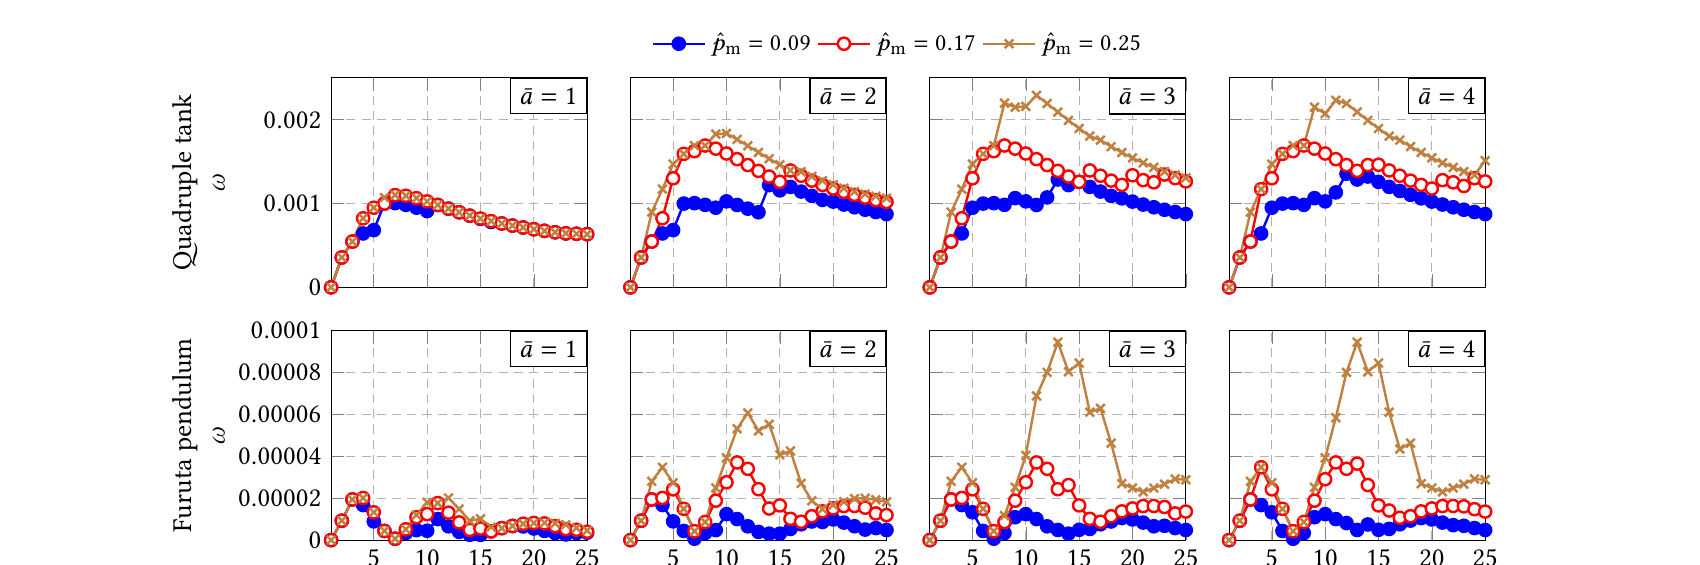
\includegraphics[width=0.9\linewidth]{../../assets/madhavi/fig2_paper.png}\\[-1pt]
  \citefig{2}
  \par\medskip
  \discuss{x-axis is attack length $\ell$ (1--25); columns are $\bar a = 1$--$4$; top row the quadruple tank (HOLD), bottom the Furuta (ZERO). $\omega$ peaks around $\ell \approx 10$ --- longer attacks are not always worse --- and raising $\bar a$ beyond 3 barely changes the impact.}
  \hook{the watchdog saturates by $\bar a \approx 3$, so a realistic threshold cannot stop this --- we optimise the DEFENCE configuration instead.}
\end{frame}

% ---------- 6. FIGURE 3 ----------
\begin{frame}{Figure 3 --- detector comparison}{binomial vs combined vs geometric ($\chi^2$) $\cdot$ $\bar a = 4$, $n_w = 20$}
  \begin{columns}[T]
    \begin{column}{0.40\textwidth}
      \centering
      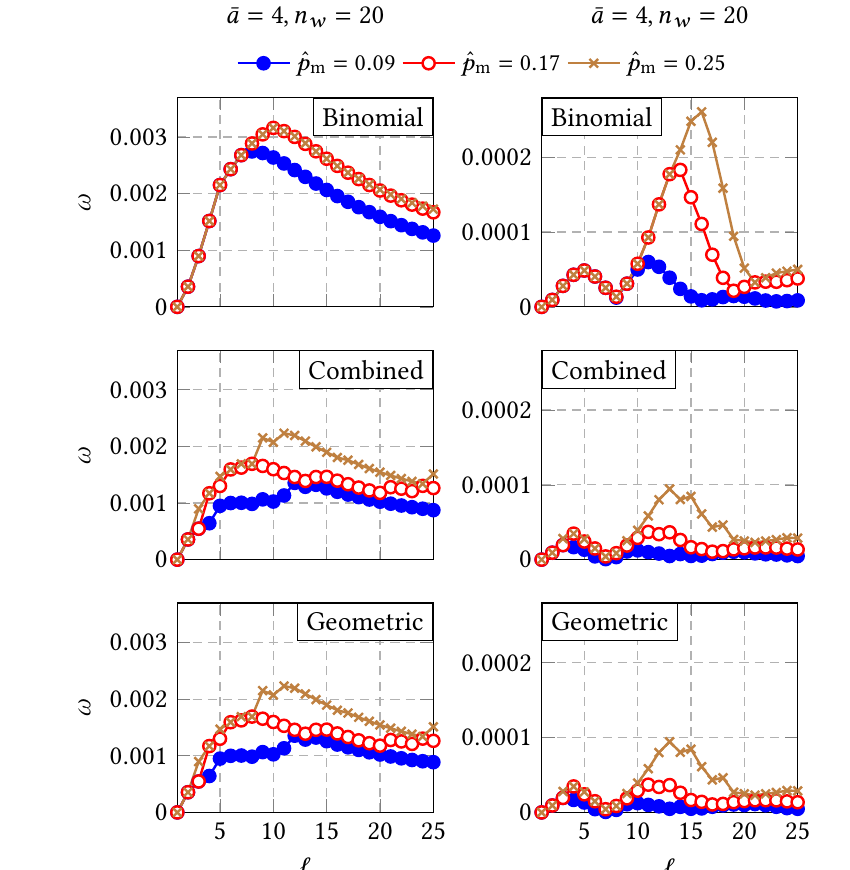
\includegraphics[height=0.74\textheight]{../../assets/madhavi/fig3_paper.png}\\[-1pt]
      \citefig{3}
    \end{column}
    \begin{column}{0.58\textwidth}
      \textbf{\textcolor{navy}{Read it}}
      \begin{itemize}\footnotesize
        \item Rows: binomial, combined, geometric detector.
        \item Left column = quadruple tank (HOLD); right = Furuta (ZERO).
        \item x-axis $= \ell$; curves for $\hat p_{\mathrm m} = 0.09/0.17/0.25$.
        \item Geometric ($\chi^2$) and combined limit the attacker \textbf{more} than binomial alone.
        \item The long-term $\chi^2$ test catches rare long bursts the short window misses.
      \end{itemize}
      \hook{$\chi^2$ is the strongest single detector --- our extension stacks multiple simultaneous windows + combined detection to push $\omega$ lower still.}
    \end{column}
  \end{columns}
\end{frame}

% ---------- 7. FIGURE 4 ----------
\begin{frame}{Figure 4 --- ZERO vs HOLD (Furuta)}{varying window $n_w = 10$--$18$ $\cdot$ $\bar a = 4$ $\cdot$ binomial detector}
  \centering
  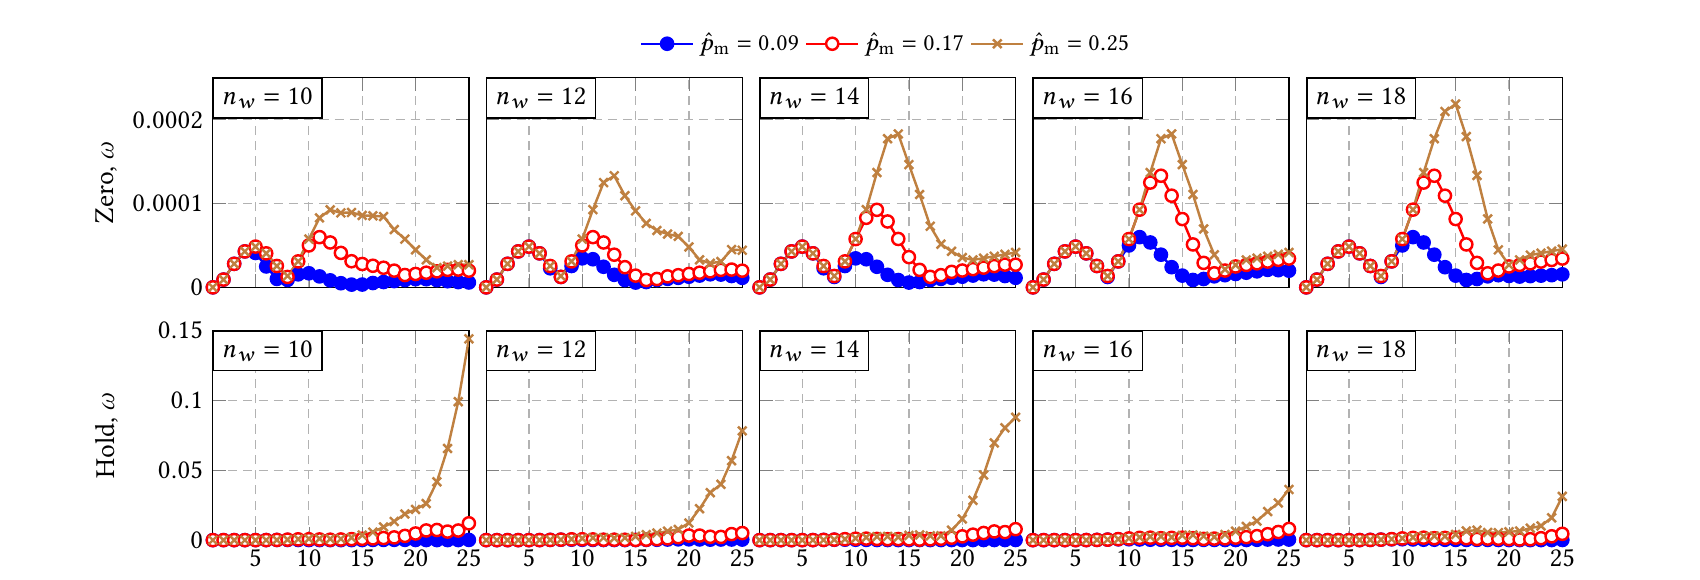
\includegraphics[width=0.9\linewidth]{../../assets/madhavi/fig4_paper.png}\\[-1pt]
  \citefig{4}
  \par\medskip
  \discuss{Top row ZERO ($\omega \approx 2\times10^{-4}$); bottom row HOLD ($\omega$ up to $0.15$ --- note the far larger scale). Under HOLD a well-timed late burst \textbf{destabilises} the pendulum; ZERO keeps $\omega$ tiny. Shorter windows help HOLD; longer windows permit longer bursts.}
  \hook{the safe policy is plant-dependent --- our defender sweep picks the policy + threshold that minimise worst-case $\omega$.}
\end{frame}

% ---------- 8. TABLE 1 ----------
\begin{frame}{Table 1 --- optimised attack sequences}{Furuta HOLD $\cdot$ $\hat p_{\mathrm m} = 0.25$, $\bar a = 4$, $\ell = 25$ $\cdot$ varying window $n_w$}
  \centering
  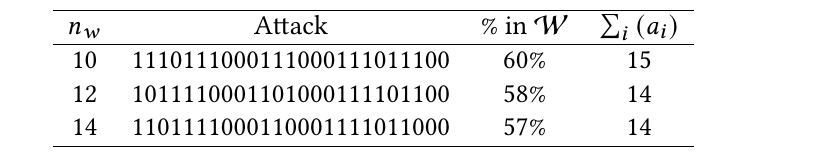
\includegraphics[width=0.62\linewidth]{../../assets/madhavi/table1_paper.png}\\[-1pt]
  {\color{muted}\tiny Table 1 $\cdot$ \copyright\ ACM --- Nauta, Sandberg \& Maggio, ICCPS 2025}
  \par\medskip
  \discuss{each row gives the optimal attack schedule, the \% of deadline misses allowed in one window (\% in $\mathcal W$), and the total misses $\sum_i a_i$. As the window widens (10$\to$14), the allowed miss density drops (60\%$\to$57\%) --- a wider window forces a sparser attack (the binomial test allows 7 misses in a window of 12, 8 in a window of 14).}
  \hook{every sequence here optimises the ATTACKER against a FIXED defence --- our novelty flips this and optimises the defence itself.}
\end{frame}

% ---------- 9. KEY FINDINGS ----------
\begin{frame}{Section 5 --- key findings}{Four results from the experiments}
  \begin{columns}[T]
    \begin{column}{0.48\textwidth}
      \begin{block}{\textcolor{white}{(i) Impact isn't monotonic in $\ell$}}
        $\omega$ peaks around $\ell \approx 10$; the optimiser concentrates or interleaves delays by initial conditions and budget.
      \end{block}
      \begin{block}{\textcolor{white}{(ii) Watchdogs barely help}}
        Effective only at $\bar a = 1$--$2$; realistic industrial thresholds (3--10) give little protection.
      \end{block}
    \end{column}
    \begin{column}{0.48\textwidth}
      \begin{block}{\textcolor{white}{(iii) $\chi^2$ dominates the binomial test}}
        The long-term run-length test limits the attacker far more than the sliding window.
      \end{block}
      \begin{block}{\textcolor{white}{(iv) ZERO beats HOLD (unstable)}}
        For the Furuta pendulum, zeroing the input on a miss is a far better defence; window length trades off per policy.
      \end{block}
    \end{column}
  \end{columns}
\end{frame}

% ---------- 10. RESULTS -> EXTENSION ----------
{\setbeamercolor{background canvas}{bg=navy}
\setbeamercolor{block title}{bg=gold,fg=navy}
\setbeamercolor{block body}{bg=navy!80!black,fg=light}
\begin{frame}[plain]
  \vskip6pt
  {\color{gold}\small\textbf{FROM THE PAPER'S RESULTS $\rightarrow$ OUR EXTENSION}}\\[0.4em]
  {\color{white}\LARGE\textbf{What the figures leave open --- and what we add}}\\[0.8em]
  \begin{columns}[T]
    \begin{column}{0.47\textwidth}
      \begin{block}{What \S5 establishes}
        \begin{itemize}\footnotesize
          \item Watchdog is weak at realistic $\bar a$ (Fig 2)
          \item $\chi^2$ is the strongest single detector (Fig 3)
          \item ZERO beats HOLD on the unstable plant (Fig 4)
          \item All optimised for a \textbf{fixed} defence (Table 1)
        \end{itemize}
      \end{block}
    \end{column}
    \begin{column}{0.47\textwidth}
      \begin{block}{Our extension (defender side)}
        \begin{itemize}\footnotesize
          \item Optimise the \textbf{defence}, not the attacker
          \item Sweep (policy, $\bar a$, window, $\hat p_{\mathrm m}$, $\alpha$) $\to \omega_{\text{worst}}$
          \item Rank configs that cap worst-case damage
          \item Multi-window detector + live visual demo
        \end{itemize}
      \end{block}
    \end{column}
  \end{columns}
  \medskip
  {\color{light}\footnotesize\textbf{\textcolor{gold}{The gap we fill:}} the paper asks ``how bad can a stealthy attacker be against a given defence?'' We answer the defender's question --- ``which defence minimises the worst stealthy attacker?'' --- and show it live.}
\end{frame}}

\end{document}
